%\documentclass{article}
%\usepackage[pdftex,active,tightpage]{preview}
%\usepackage{tikz}
%\begin{document}
%\begin{preview}
%%%%%%%%%%%%%%%%%%%%%%%%%%%%%%%%%
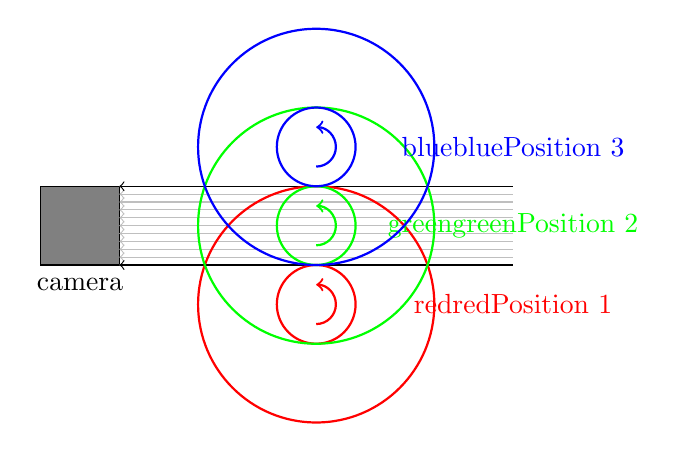
\begin{tikzpicture}
	\def\length{1}
	\def\beamlength{6}
	%camera
	\draw [fill=gray] (0,0) rectangle (\length,\length);
	\node at (.5*\length,-.25) {camera};
	% beam
	\foreach \x in {0,.1,...,1.1}
		\draw[gray!50,<-] (\length,\x) -- (\beamlength,\x);
	\foreach \x in {0,\length}
		\draw[<-] (\length,\x) -- (\beamlength,\x);
%	\node at (3.5*\length,\length+.25) {beam};
	%samples
	\foreach \y/\color/\position in {-.5/red/1,.5/green/2,1.5/blue/3}
		{
			\draw[thick,color=\color] (0.5*\beamlength+0.5*\length,\y) circle (1.5*\length) circle (.5*\length);
			\draw[thick,->,color=\color] (0.5*\beamlength+0.5*\length,\y-.25*\length) arc (-90:90:0.25*\length);
			\node[color=\color] at (\beamlength,\y) {Position \position};
		}
\end{tikzpicture}
%%%%%%%%%%%%%%%%%%%%%%%%%%%%%%%%%
%\end{preview}	
%\end{document}